\section{Experiments}
\label{sec:experiments}
\label{sec:analysis}

\iffalse
\setlength{\tabcolsep}{3pt}
\begin{table}
\scriptsize
\caption{Mean scores obtained by our method (SimPLe) in comparison with Rainbow trained on 100K steps (400K frames) and PPO trained on 500K steps (2 millions frames). Details and extended numerical results are included in Appendix~\ref{numerical_results}.}
\begin{tabular}{lrrrrr}

Game &          SimPLe (ours)  &     rainbow\_100k &     ppo\_500k   &     human &          random \\

\midrule
Alien          &    405.2 &    290.6 &    269.0 &   7128.0 &   184.8 \\
Amidar         &     88.0 &     20.8 &     93.2 &   1720.0 &    11.8 \\
Assault        &    369.3 &    300.3 &    552.3 &    742.0 &   233.7 \\
Asterix        &   1089.5 &    285.7 &   1085.0 &   8503.0 &   248.8 \\
BankHeist      &      8.2 &     34.5 &    641.0 &    753.0 &    15.0 \\
BattleZone     &   5184.4 &   3363.5 &  14400.0 &  37188.0 &  2895.0 \\
Boxing         &      9.1 &      0.9 &      3.5 &     12.0 &     0.3 \\
Breakout       &     12.7 &      3.3 &     66.1 &     30.0 &     0.9 \\
ChopperCommand &   1246.9 &    776.6 &    860.0 &   7388.0 &   671.0 \\
CrazyClimber   &  39827.8 &  12558.3 &  33420.0 &  35829.0 &  7339.5 \\
DemonAttack    &    169.5 &    431.6 &    216.5 &   1971.0 &   140.0 \\
Freeway        &     20.3 &      0.1 &     14.0 &     30.0 &     0.0 \\
Frostbite      &    254.7 &    140.1 &    214.0 &      - &    74.0 \\
Gopher         &    771.0 &    748.3 &    560.0 &   2412.0 &   245.9 \\
Hero           &   1295.1 &   2676.3 &   1824.0 &  30826.0 &   224.6 \\
Jamesbond      &    125.3 &     61.7 &    255.0 &    303.0 &    29.2 \\
Kangaroo       &    323.1 &     38.7 &    340.0 &   3035.0 &    42.0 \\
Krull          &   4539.9 &   2978.8 &   3056.1 &   2666.0 &  1543.3 \\
KungFuMaster   &  17257.2 &   1019.4 &  17370.0 &  22736.0 &   616.5 \\
MsPacman       &    762.8 &    364.3 &    306.0 &   6952.0 &   235.2 \\
Pong           &      5.2 &    -19.5 &     -8.6 &     15.0 &   -20.4 \\
PrivateEye     &     58.3 &     42.1 &     20.0 &  69571.0 &    26.6 \\
Qbert          &    559.8 &    235.6 &    757.5 &  13455.0 &   166.1 \\
RoadRunner     &   5169.4 &    524.1 &   5750.0 &   7845.0 &     0.0 \\
Seaquest       &    370.9 &    206.3 &    692.0 &  42055.0 &    61.1 \\
UpNDown        &   2152.6 &   1346.3 &  12126.0 &  11693.0 &   488.4 \\
\bottomrule
\end{tabular}
\label{tab:shortNumericalResults}
\end{table}
\fi

We evaluate SimPLe on a suite of Atari games from Atari Learning Environment (ALE) benchmark.
In our experiments, the training loop is repeated for 15 iterations, with $6400$ interactions with the environment collected in each iteration.
We apply a standard pre-processing for Atari games: a frame skip equal to 4, that is every action
is repeated 4 times. The frames are down-scaled by a factor of $2$.

Because some data is collected before the first iteration of the loop,
altogether $6400 \cdot 16 = 102,400$ interactions with the Atari environment are used during training.
This is equivalent to $409,600$ frames from the Atari game (114 minutes at 60 FPS).
At every iteration, the latest policy trained under the learned model is used to collect data in the real environment $\env$.
% BO 2020/02/12.
The data is also directly used to train the policy with PPO.
Due to vast difference between number of training data from simulated environment and real environment (15M vs 100K) the impact of the latter on policy is negligible.
% as part of the Tensor2Tensor library with instructions on how to run our experiments.\footnote{\url{https://github.com/tensorflow/tensor2tensor/tree/master/tensor2tensor/rl}} 

We evaluate our method on $26$ games selected on the basis of being solvable with existing state-of-the-art model-free deep RL algorithms\footnote{Specifically, for the final evaluation we selected games which achieved non-random results using our method or the Rainbow algorithm using $100$K interactions.}, which in our comparisons are Rainbow~\cite{rainbow} and PPO~\cite{ppo}. For Rainbow, we used the implementation from the Dopamine package and spent considerable time tuning it for sample efficiency (see Appendix \ref{sec:baselines_optimizations}).

For visualization of all experiments see \url{https://goo.gl/itykP8}
and for a summary see Figure~\ref{fig:compare_dopamine_ppo}.
It can be seen that our method is more sample-efficient than a highly tuned Rainbow baseline on almost all games, requires less than half of the samples on more than half of the games and, on {\freeway}, is more than 10x more sample-efficient. Our method outperforms PPO by an even larger margin.
We also compare our method with fixed score baselines (for different baselines) rather than counting how many steps are required to match our score, see Figure~\ref{fig:compare_scores} for the results.
For the qualitative analysis of performance on different games see Appendix \ref{qualitative_analysis}.
The source code is available as part of the Tensor2Tensor library and it includes instructions on how to run the experiments\footnote{\url{https://github.com/tensorflow/tensor2tensor/tree/master/tensor2tensor/rl}}.

\begin{figure}
\centering
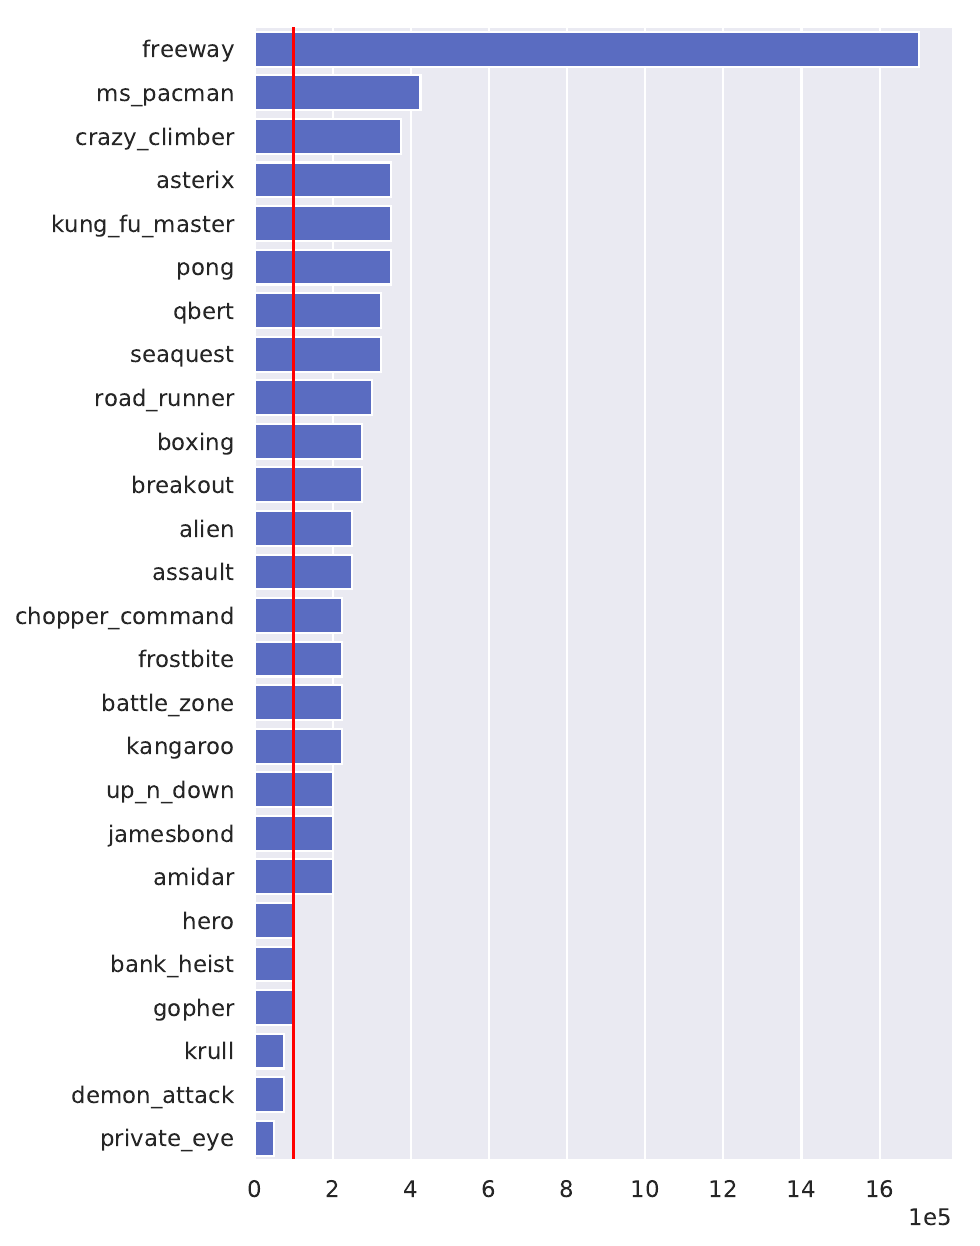
\includegraphics[width=0.45\columnwidth]{figures/v1_eval_longmodel_vs_rainbow-1.png}
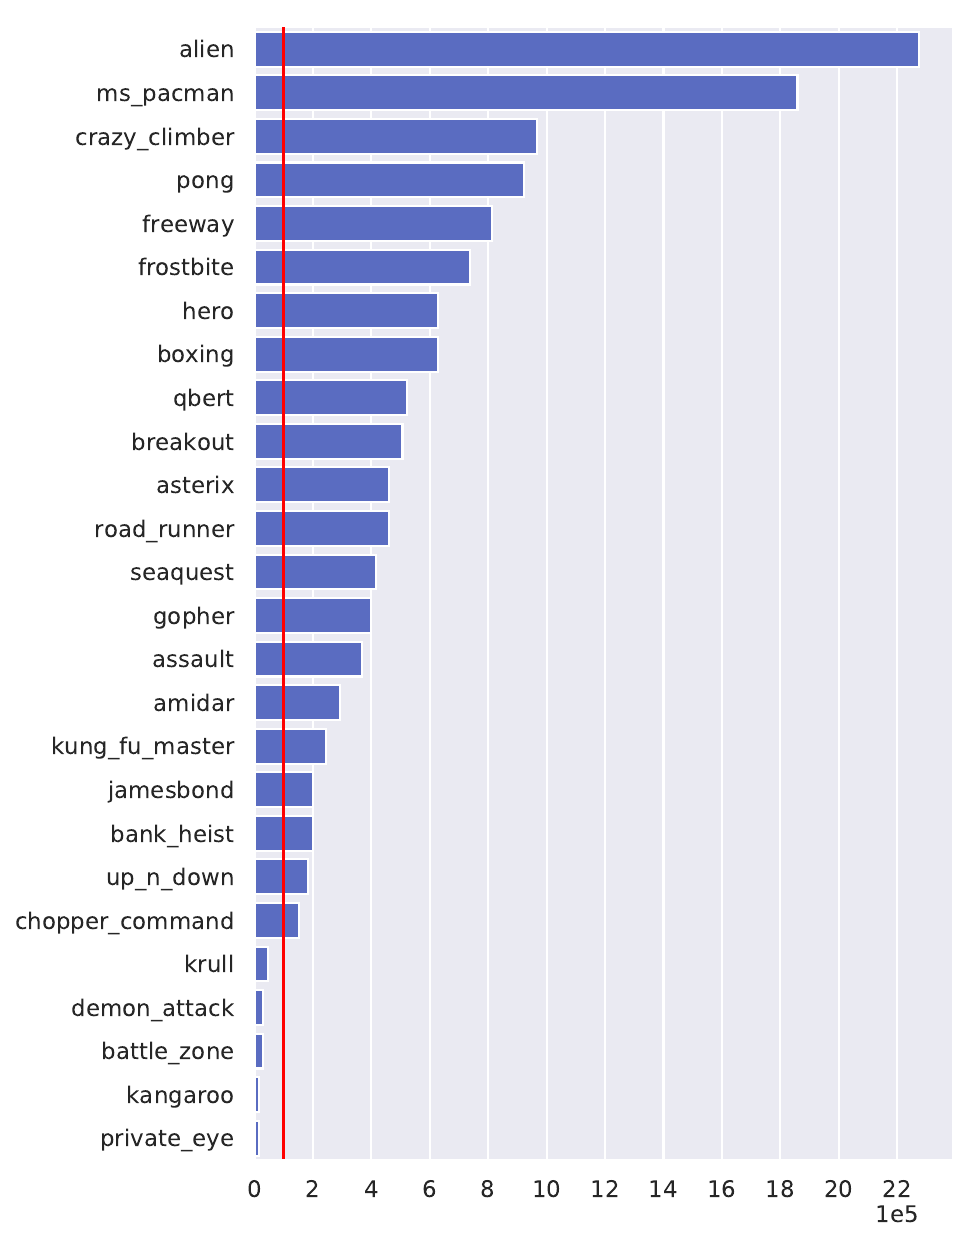
\includegraphics[width=0.45\columnwidth]{figures/v1_eval_longmodel_vs_ppo-1.png}
\vspace{-0.2cm}
\caption{Comparison with Rainbow and PPO. Each bar illustrates the number of interactions with environment required by Rainbow (left) or PPO (right) to achieve the same score as our method (SimPLe). The red line indicates the $100$K interactions threshold which is used by the our method.} 
\label{fig:compare_dopamine_ppo}
\vspace{-0.5cm}
\end{figure}


\subsection{Sample Efficiency}
The primary evaluation in our experiments studies the sample efficiency of SimPLe, in comparison with state-of-the-art model-free deep RL methods in the literature. To that end, we compare with  Rainbow~\citep{rainbow,DBLP:journals/corr/abs-1812-06110}, which represents the state-of-the-art Q-learning method for Atari games, and PPO~\citep{ppo}, a model-free policy gradient algorithm (see Appendix \ref{sec:baselines_optimizations} for details of tuning of Rainbow and PPO). The results of the comparison are presented in Figure~\ref{fig:compare_dopamine_ppo}. For each game, we plot the number of time steps needed for either Rainbow or PPO to reach the same score that our method reaches after $100$K interaction steps. The red line indicates $100$K steps: any bar larger than this indicates a game where the model-free method required more steps. SimPLe outperforms the model-free algorithms in terms of learning speed on nearly all of the games, and in the case of a few games, does so by over an order of magnitude. For some games, it reaches the same performance that our PPO implementation reaches at $10$M steps. This indicates that model-based reinforcement learning provides an effective approach to learning Atari games, at a fraction of the sample complexity.

The results in these figures % and Table \ref{tab:shortNumericalResults}
are generated by averaging $5$ runs for each game.
% As shown in Table \ref{tab:shortNumericalResults},
The model-based agent is better than a random policy for all the games except \bankh. Interestingly, we observed that the best of the $5$ runs was often significantly better. For $6$ of the games, it exceeds the average human score (as reported in Table 3 of \cite{Pohlenetal2018}). This suggests that further stabilizing SimPLe should improve its performance, indicating an important direction for future work. In some cases during training  we observed high variance of the results during each step of the loop. There are a number of possible reasons, such as mutual interactions of the policy training and the supervised training or domain mismatch between the model and the real environment. We present detailed numerical results, including best scores and standard deviations, in Appendix \ref{numerical_results}.

\begin{figure}
\centering
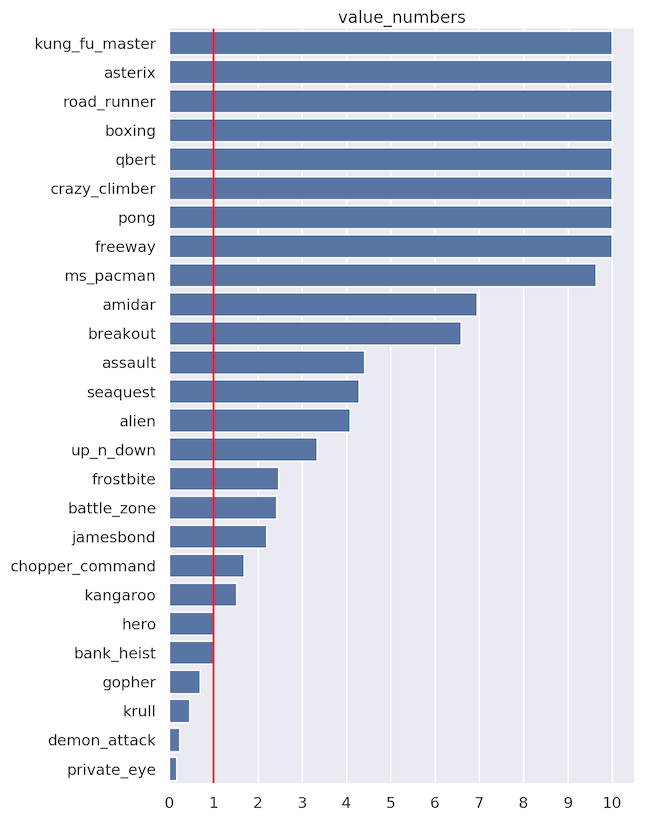
\includegraphics[width=0.245\columnwidth]{figures/nfraction_of_rainbow_at_100K.png}
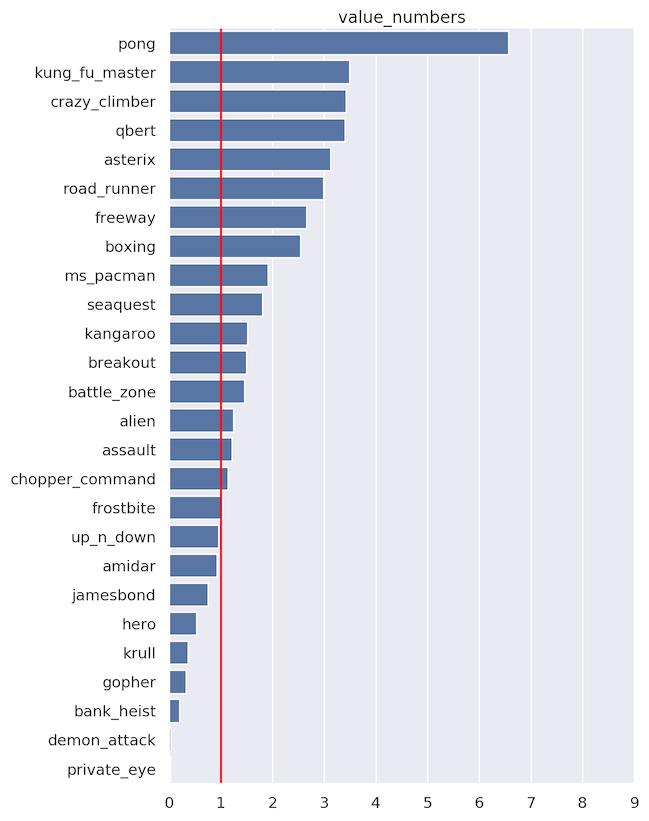
\includegraphics[width=0.245\columnwidth]{figures/nfraction_of_rainbow_at_200K.png}
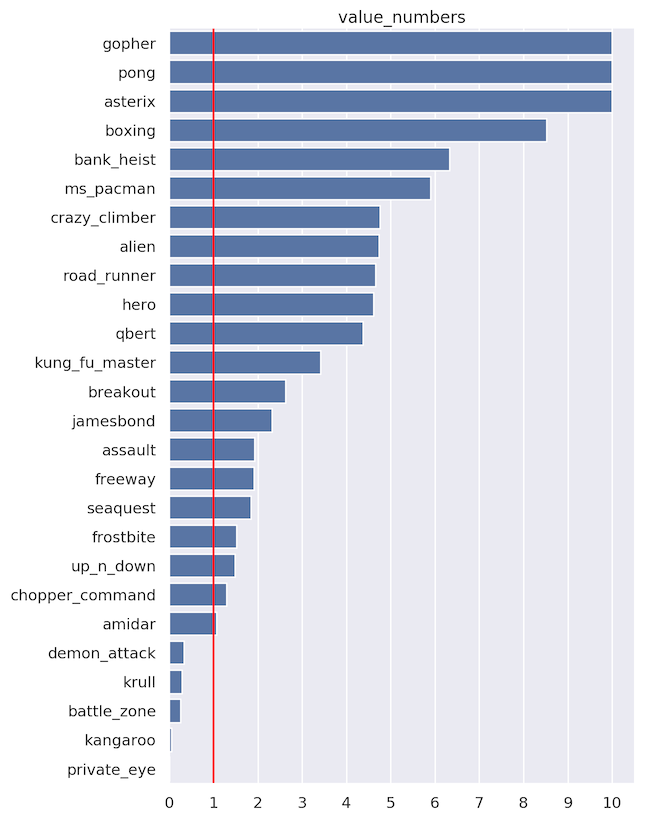
\includegraphics[width=0.245\columnwidth]{figures/nfraction_of_ppo_at_100K.png}
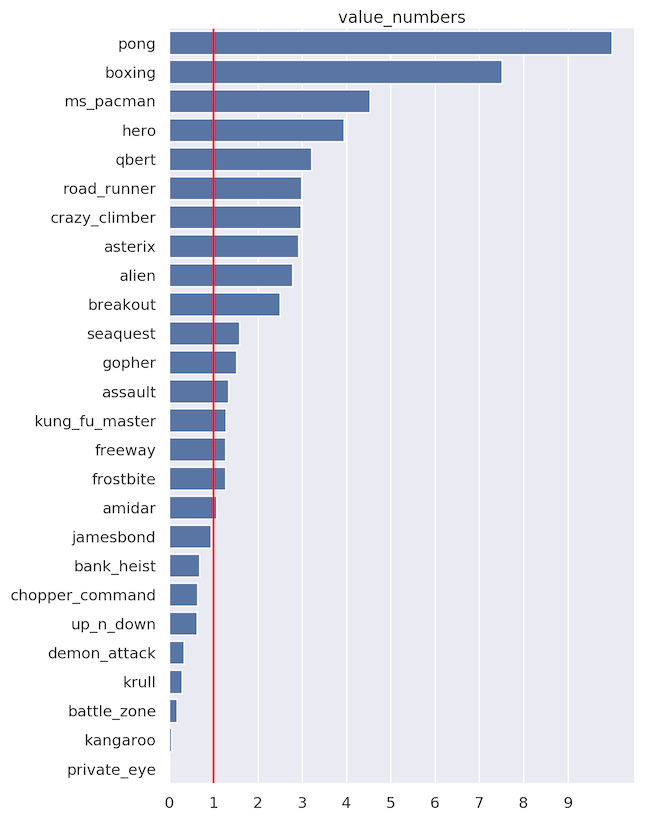
\includegraphics[width=0.245\columnwidth]{figures/nfraction_of_ppo_at_200K.png}
\vspace{-0.2cm}
\caption{Fractions of Rainbow and PPO scores at different numbers of interactions calculated with the formula $(SimPLe\_score@100K - random\_score)/(baseline\_score - random\_score)$; if denominator is smaller than 0, both nominator and denominator are increased by 1. From left to right, the baselines are: Rainbow at 100K, Rainbow at 200K, PPO at 100K, PPO at 200K.
SimPLe outperforms Rainbow and PPO even when those are given twice as many interactions.}
\label{fig:compare_scores}
\vspace{-0.5cm}
\end{figure}

\subsection{Number of frames}

We focused our work on learning games with $100$K interaction steps with the environment. In this section we present additional results for settings with $20$K, $50$K, $200$K, $500$K and $1$M interactions; see Figure~\ref{fig:numberOfStepsMT}~(a).
Our results are poor with $20$K interactions. For $50$K they are already almost as good as with $100$K interactions. From there the results improve until $500$K samples -- it is also the point at which they are on par with model-free PPO. Detailed per game results can be found in Appendix~\ref{appdx:num_samples}.

This demonstrates that SimPLe excels in a low data regime, but its advantage disappears with a bigger amount of data.
Such a behavior, with fast growth at the beginning of training, but lower asymptotic performance is commonly observed when comparing model-based and model-free methods (\citet{benchmarkingmbrl}). As observed in Section \ref{subabl} assigning bigger computational budget helps in $100$K setting. We suspect that gains would be even bigger for the settings with more samples. 
% The limitation of the presented results is that even with the highest number of frames, the method was assigned the same computational budget as for $100$K interactions. As suggested by Section \ref{subabl}, we could expect further improvement to the performance with prolonging model training.

Finally, we verified if a model obtained with SimPLe using $100$K is a useful initialization for model-free PPO training. 
Based on the results depicted in Figure~\ref{fig:numberOfStepsMT}~(b) we can positively answer this conjecture. Lower asymptotic performance is probably due to worse exploration. A policy pre-trained with SimPLe was meant to obtain the best performance on $100$K, at which point its entropy is very low thus hindering further PPO training.

\newcommand{\mywidth}{3.5in}
\begin{figure}
\begin{tabular}{@{\hskip -3em}c@{\hskip -3.5em}c}
\subfloat[Model based (SimPLe)]{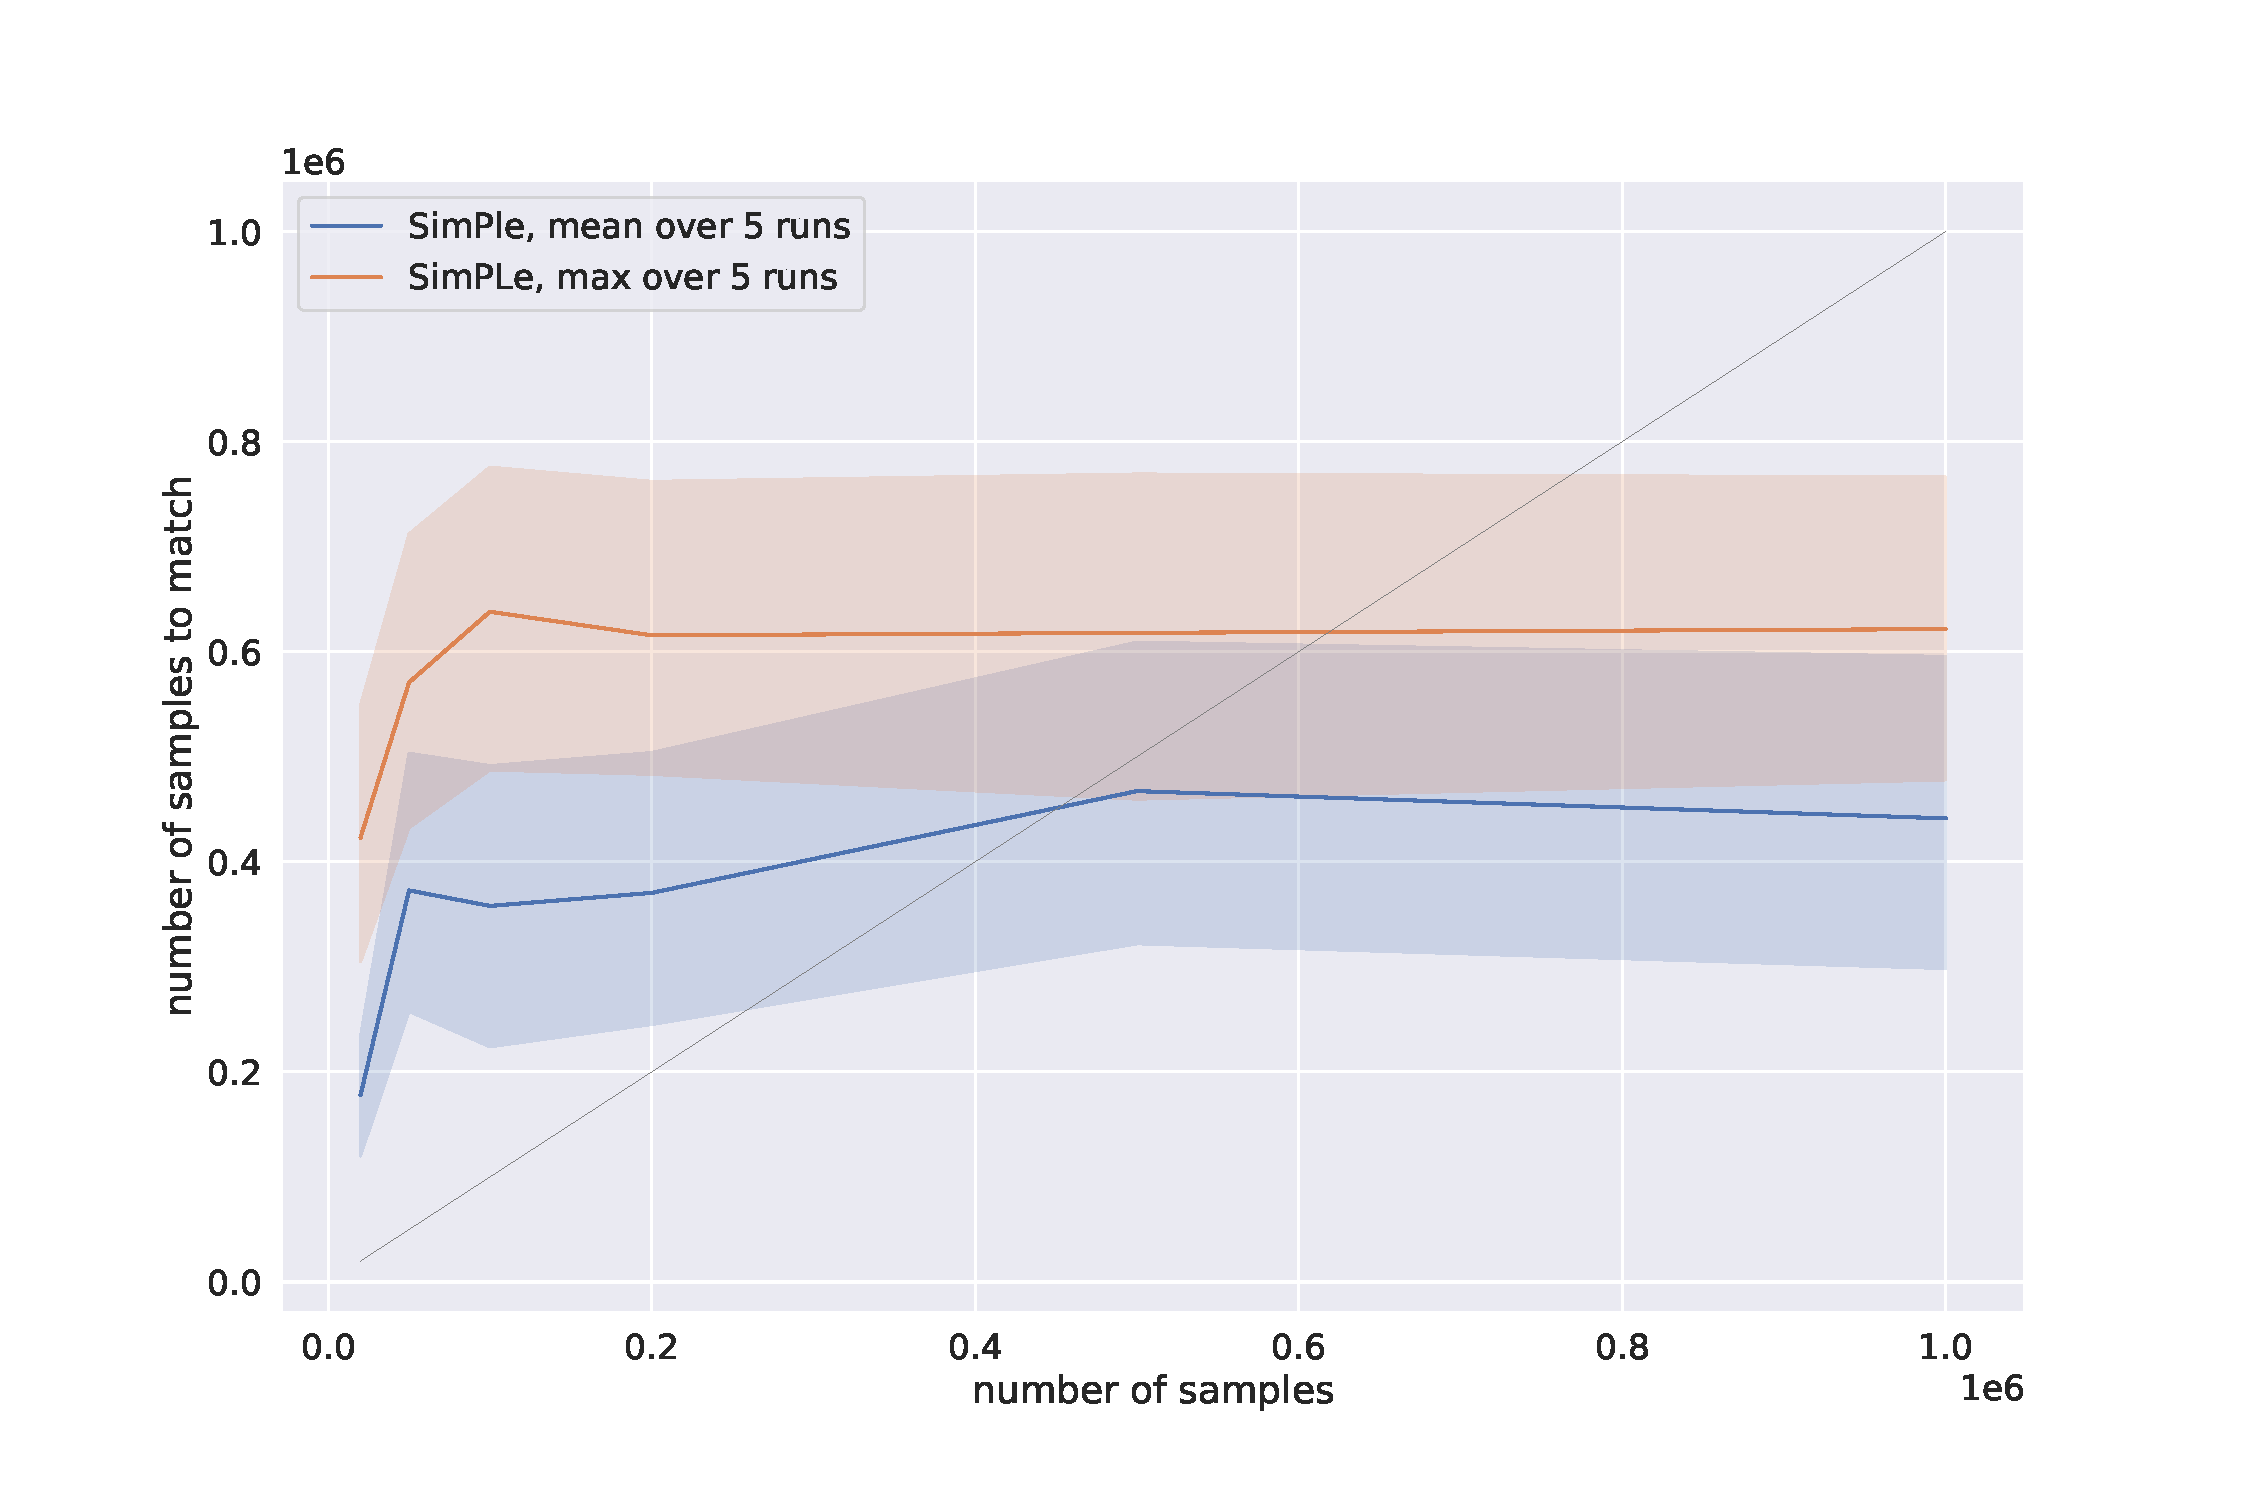
\includegraphics[width = \mywidth ]{figures/number_of_step_simple.pdf}} &
\subfloat[Model based + model free (SimPLe + PPO)]{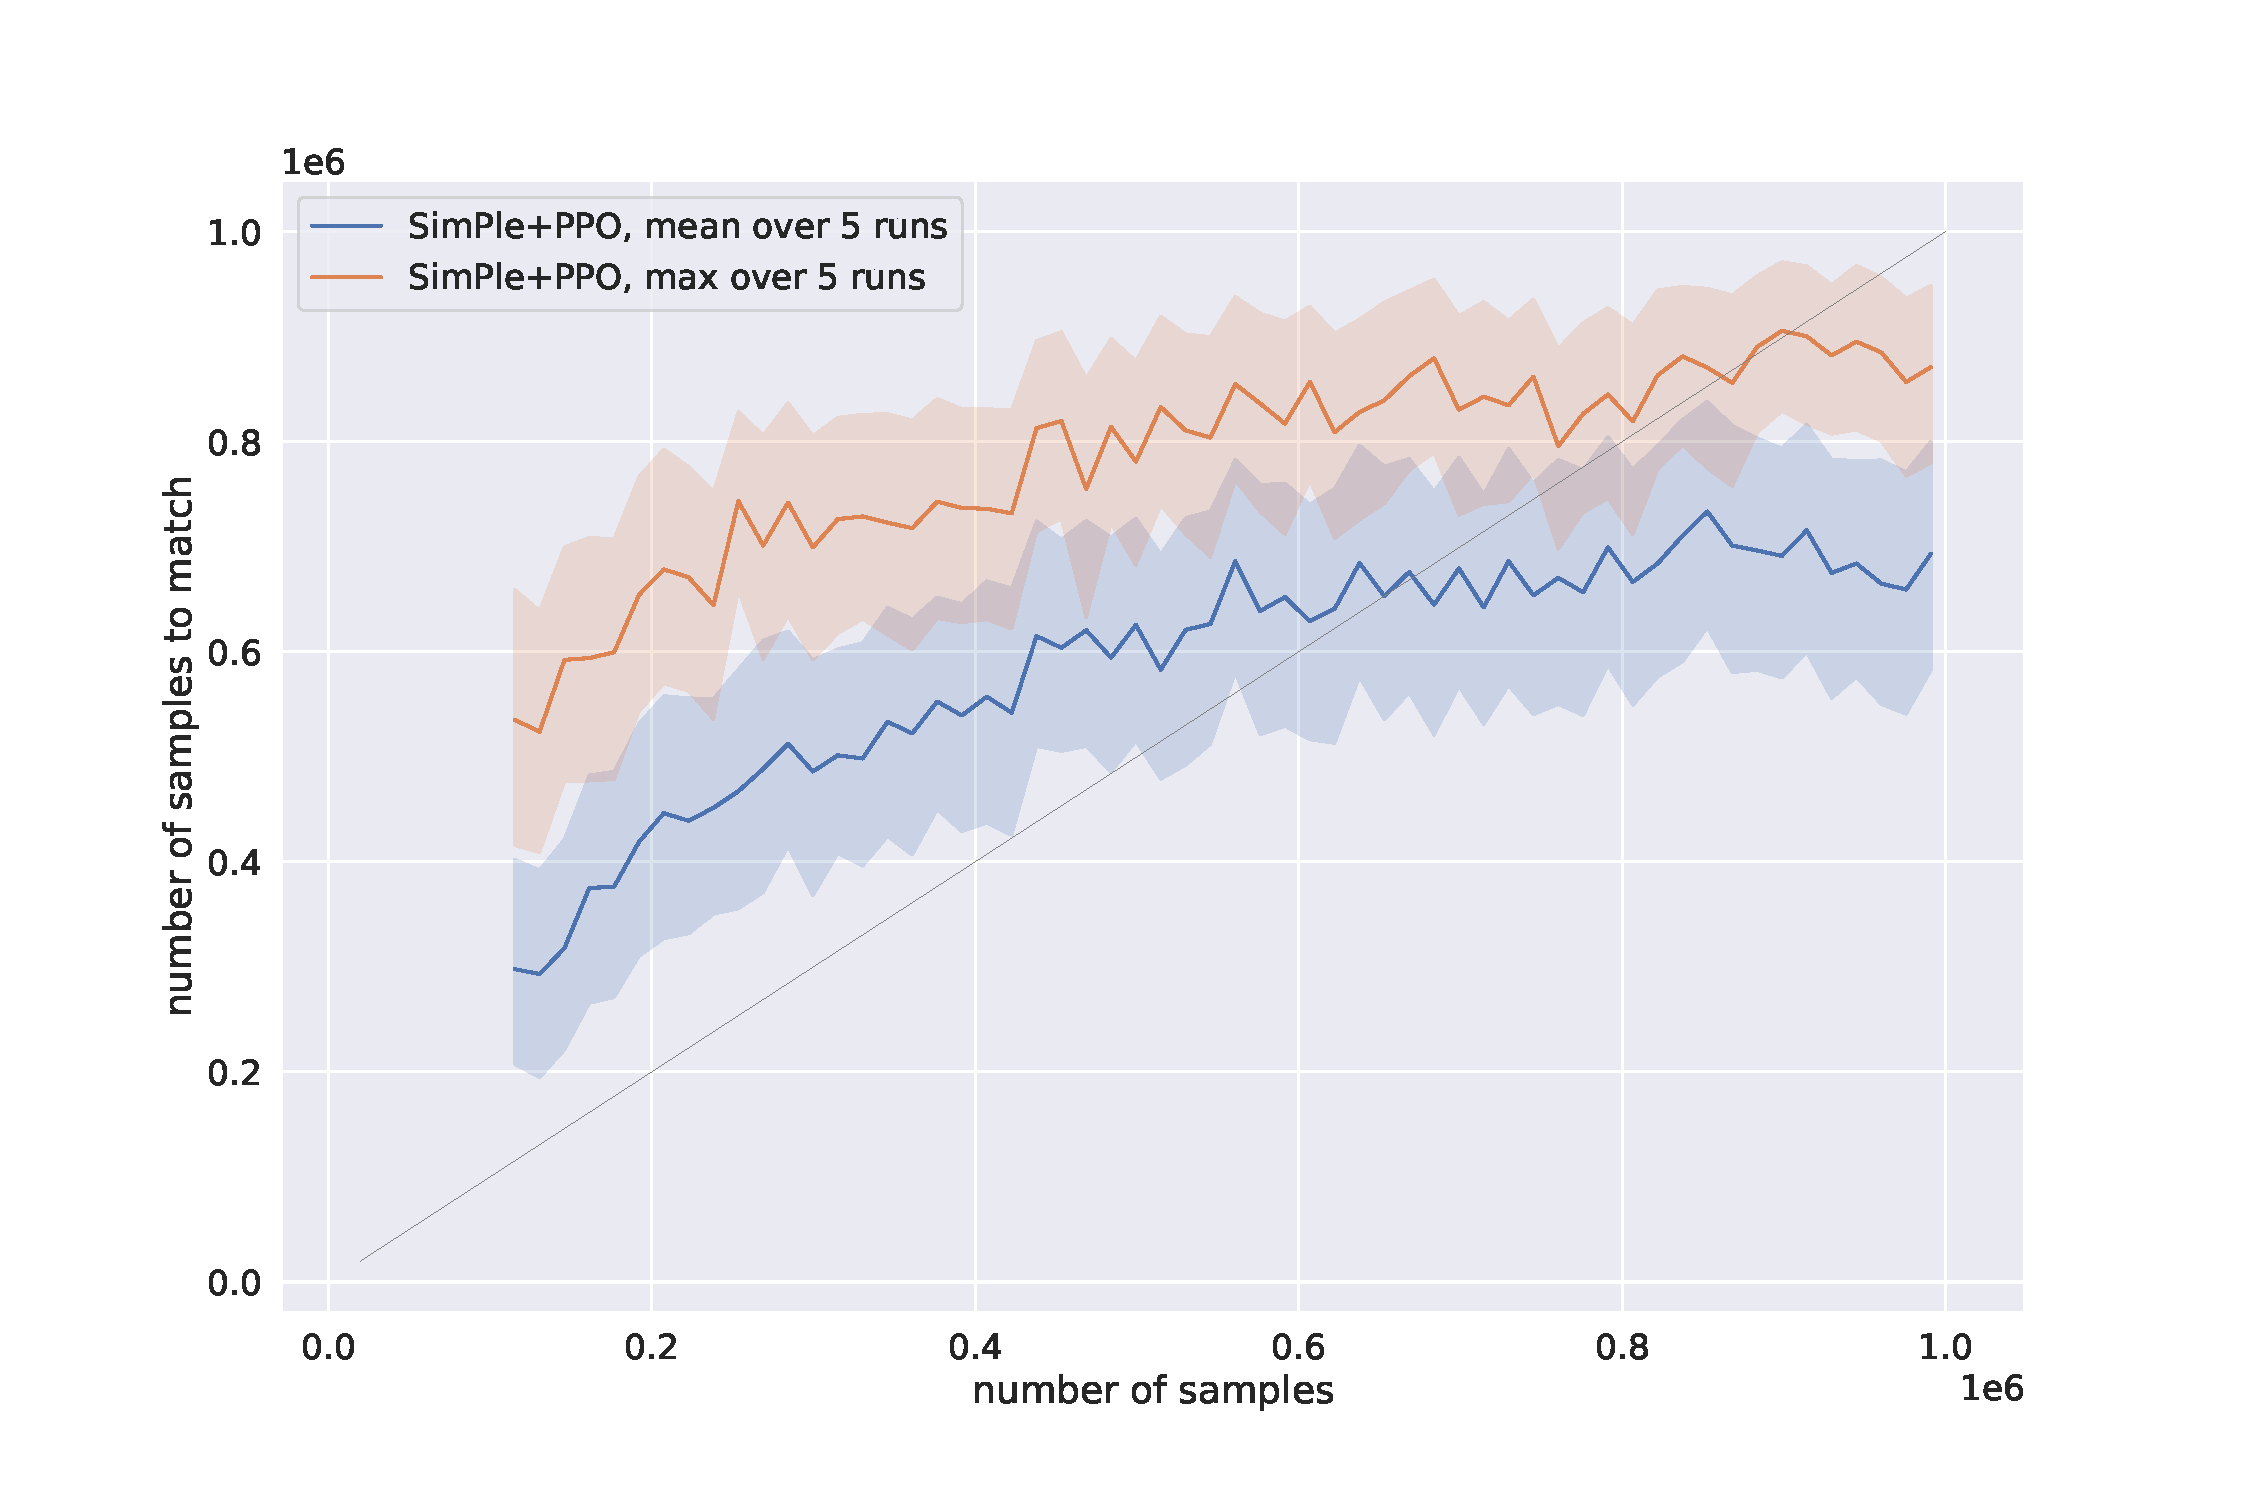
\includegraphics[width = \mywidth]{figures/number_of_step_simple_ppo.pdf}} 
\end{tabular}
\caption{Behaviour with respect to the number of used samples. We report number of frames required by PPO to reach the score of our models. Results are averaged over all games.\label{fig:numberOfStepsMT}}
\end{figure}

\subsection{Environment stochasticity}

A crucial decision in the design of world models is the inclusion of stochasticity. Although Atari is known to be a deterministic environment, it is stochastic given only a limited horizon of past observed frames (in our case $4$ frames). The level of stochasticity is game dependent; however, it can be observed in many Atari games.
% BO 2020/02/12
%An example of such behavior can be observed in the game \texttt{Kung Fu Master} -- after eliminating current set of opponents the game screen always looks the same (i.e. contains only player's character and the background). Based on this observation alone (and not the game internal state) it is most likely impossible to predict which opponents will emerge from behind the screen edge. A fully deterministic model would be bound to fail -- it could either keep predicting empty frames, or predict the same set of opponents, or a blurred image which average all potential opponents. As can be seen in Figure~\ref{fig:kungfu} in the Appendix the stochastic model learns a reasonable behavior -- samples potential opponents and renders them sharply.
An example of such behavior can be observed in the game \texttt{Kung Fu Master} -- after eliminating the current set of opponents, the game screen always looks the same (it contains only player's character and the background). The game dispatches diverse sets of new opponents, which cannot be inferred from the visual observation alone (without access to the game's internal state) and thus cannot be predicted by a deterministic model. Similar issues have been reported in \cite{sv2p}, where the output of their baseline deterministic model was a blurred superposition of possible random object movements. As can be seen in Figure~\ref{fig:kungfu} in the Appendix, the stochastic model learns a reasonable behavior -- samples potential opponents and renders them sharply.

\begin{wrapfigure}[26]{r}{0.45\textwidth}\label{fig:sticky}
\vspace{-0.5cm}
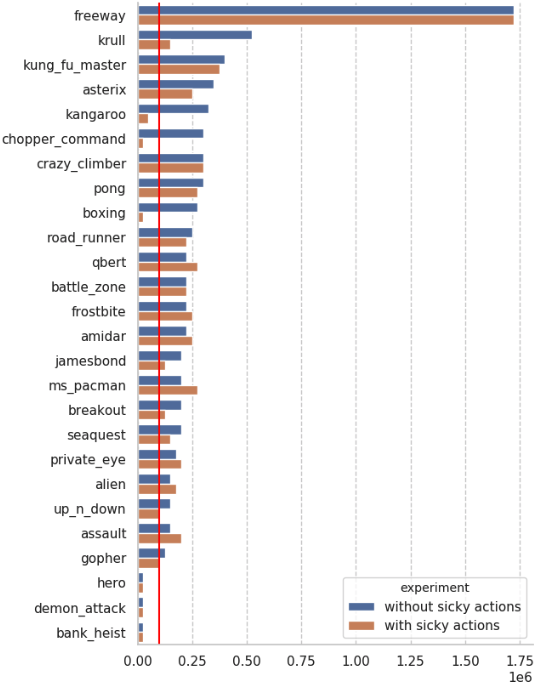
\includegraphics[width=0.45\textwidth]{figures/sticky_2}
%\vspace{-0.2cm}
\caption{Impact of the environment stochasticity.
%Comparison of experiments with and without sticky actions using stochastic discrete world models.
The graphs are in the same format as Figure~\ref{fig:compare_dopamine_ppo}: each bar illustrates the number of interactions with environment required by Rainbow to achieve the same score as SimPLe (with stochastic discrete world model) using 100k steps in an environment with and without sticky actions.}
\label{fig:sticky}
\end{wrapfigure}

Given the stochasticity of the proposed model, SimPLe can be used with truly stochastic environments. To demonstrate this, we ran an experiment where the full pipeline (both the world model and the policy) was trained in the presence of sticky actions, as recommended in \cite[Section 5]{ale2}. Our world model learned to account for the stickiness of actions and in most cases the end results were very similar to the ones for the deterministic case even without any tuning, see Figure~\ref{fig:sticky}.

\subsection{Ablations}\label{subabl}
To evaluate the design of our method, we independently varied a number of the design decisions. Here we present an overview; see Appendix~\ref{sec:ablations} for detailed results.
\vspace{0.1cm}\\\textbf{Model architecture and hyperparameters.}
We evaluated a few choices for the world model and our proposed stochastic discrete model performs best by a significant margin.
The second most important parameter was the length of world model's training. We verified that a longer training would be beneficial,
%but we had to restrict it because of a high cost of running the whole training on all Atari games.
however we had to restrict it in all other ablation studies due to a high cost of training on all games.
% but due to our resources constraints other ablations because were made with the short model training setting.
As for the length of rollouts from simulated $env'$, we use $N=50$ by default. We experimentally shown that $N=25$ performs roughly on par, while $N=100$ is slightly worse, likely due to compounding model errors.
%We experimented with $N=25$ or $N=100$ and $100$ is a bit worse than either $25$ or $50$ (which are on par), likely due to compounding model errors, but this effect is much smaller than the effect of model architecture.
The \emph{discount factor} was set to $\gamma=0.99$ unless specified otherwise.  We see that $\gamma=0.95$ is slightly better than other values, and we hypothesize that it is due to better tolerance to model imperfections. But overall, all three values of $\gamma$ perform comparably.
\vspace{0.1cm}\\\textbf{Model-based iterations.}
The iterative process of training the model, training the policy, and collecting data is crucial for non-trivial tasks where random data collection is insufficient. In a game-by-game analysis, we quantified the number of games where the best results were obtained in later iterations of training. In some games, good policies could be learned very early. While this might have been due to the high variability of training, it does suggest the possibility of much faster training (i.e. in fewer step than 100k) with more directed exploration policies. In Figure \ref{fig:Cdf} in the Appendix we present the cumulative distribution plot for the (first) point during learning when the maximum score for the run was achieved in the main training loop of Algorithm~\ref{alg:basic_loop}.
\vspace{0.1cm}\\\textbf{Random starts.} Using short rollouts is crucial to mitigate the compounding errors in the model. To ensure exploration, SimPLe starts rollouts from randomly selected states taken from the real data buffer $\textsc{D}$. Figure \ref{fig:Cdf} compares the baseline with an experiment without random starts and rollouts of length $1000$ on {\seaquest} which shows much worse results without random starts.

% \subsection{Qualitative Analysis}
% In addition to ablating parameters, we studied of individual games to better understand how SimPLe works. We emphasize that we did not adjust the method nor hyperparameters individually for each game, but we provide specific qualitative analysis to better understand our models.\footnote{We strongly encourage the reader to watch accompanying videos \url{https://goo.gl/itykP8}} 

% In some games (\pong, \freeway, \breakout) our models were able to predict the future pixel-perfect. In some other cases our models differed from the original games in a way that was harmless for policy training. For example, in {\bowling}, and {\pong}, the ball sometimes splits into two. While nonphysical, seemingly these errors did not distort much the objective of the game.

% In {\kungfumaster}, our model's predictions deviate from the real game by spawning a different number of opponents. In {\crazyclimber}, we observed the bird appearing earlier in the game. We attribute these cases to the stochasticity in the model. Though not aligned with the true environment, the predicted behaviors are plausible and the resulting policy can still play the original game.

% Finally, on some of the games, our models simply failed to produce useful predictions. The most common failure was due to the presence of very small but highly relevant objects. For example, in {\atlantis} and {\battlezone} bullets are so small that they tend to disappear. In Appendix~\ref{qualitative_analysis} we provide more detailed analysis.
